\section{verwendete Messgeräte \& Entwicklungstools}
\subsection{DE10-Lite Board}
\begin{tabular}[h]{l|l}
	Art & DE-Lite Board\\
	\hline
	Produktnummer & DE10-Lite\\
	\hline
	Seriennummer & 19040005-1757\\
	\hline
	TGM Inv. Nr. & Eigentum Sauer\\
	\hline
	Beschreibung & FPGA-Entwicklungsplatine\\
	& Chip: Max 10 10M50DAF484C7G\\
	& 50 MHz\\
	& Power Supply: 5V USB\\
	\hline
	Foto & \raisebox{-\height}{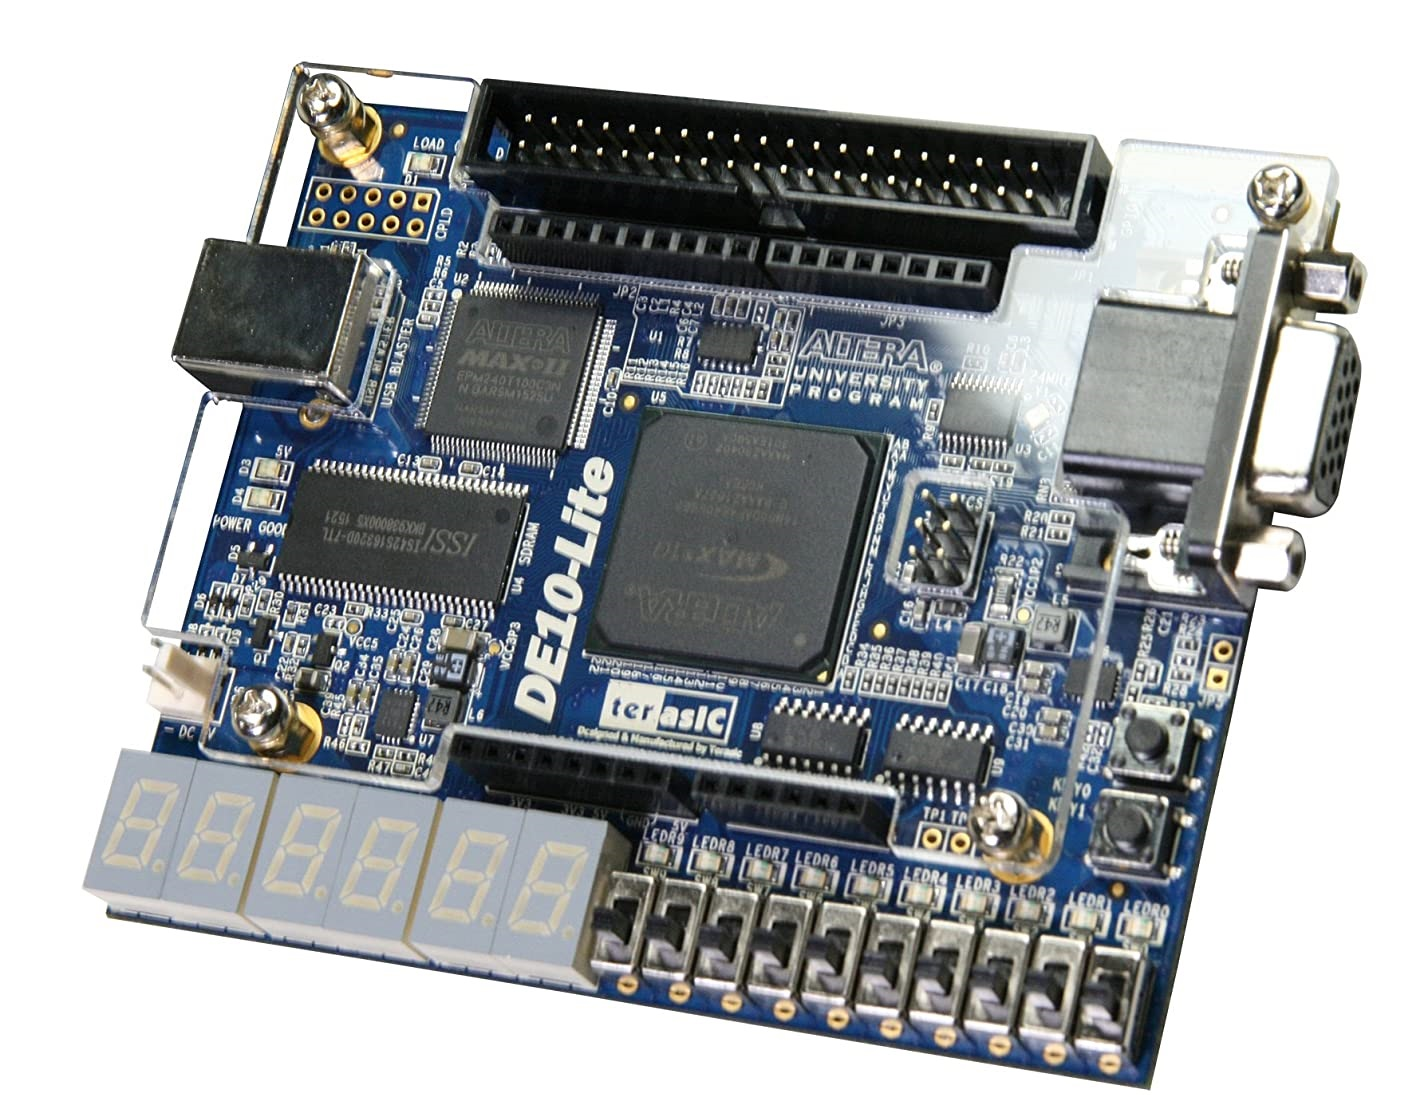
\includegraphics[width=8cm,angle=0]{Geraete/DE10-Lite.jpg}}\\
\end{tabular}
\subsection{Oszilloskop 1} \label{Oszi1}
\begin{tabular}[h]{l|l}
Art & Oszilloskop\\
\hline
Produktnummer & HM1507-2\\
\hline
Seriennummer & /\\
\hline
TGM Inv. Nr. & 540-16/22/99\\
\hline
Beschreibung & digitales Oszilloskop\\
 & 2 Channel\\
 & 150 MHz | 200 MSa/s\\
 & Röhrenbildschirm\\
\hline
Foto & \raisebox{-\height}{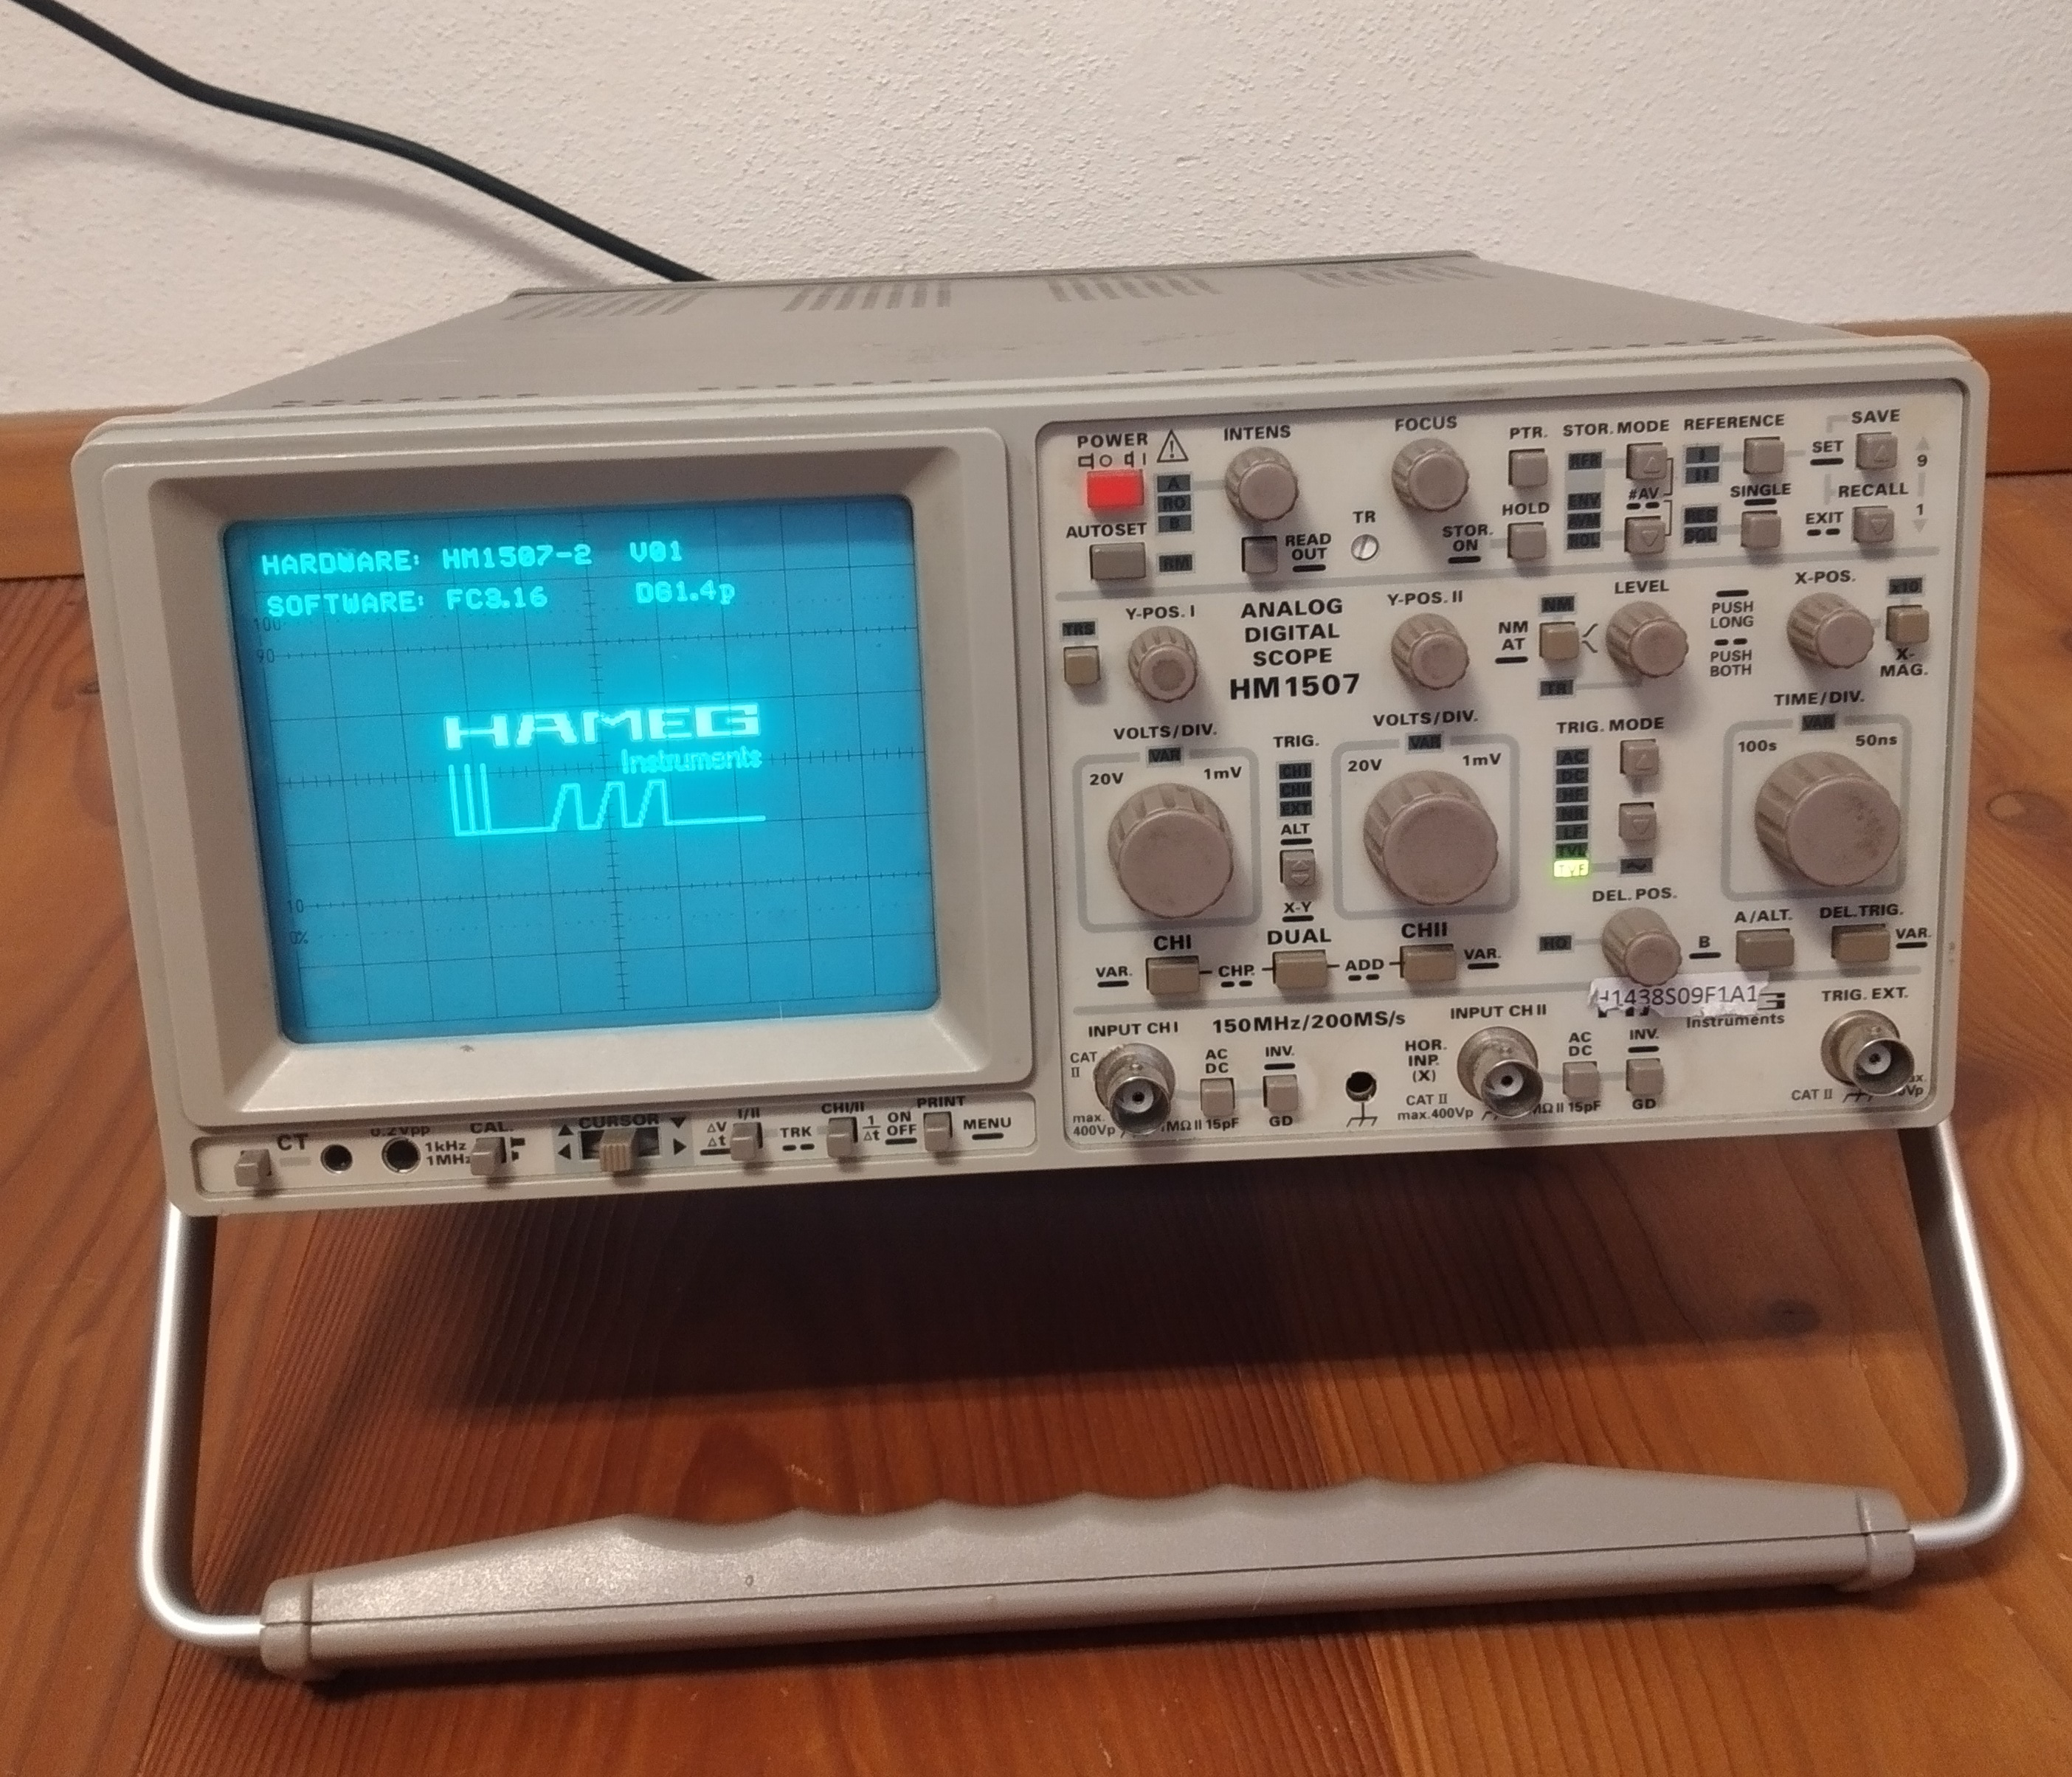
\includegraphics[width=8cm,angle=0]{Geraete/Oszi1.jpg}}\\
\end{tabular}

\subsection{RS232-Adapter} \label{RS232-Adapter}
\begin{tabular}[h]{l|l}
	Art & RS232-Adapter\\
	\hline
	Produktnummer & AU0002E\\
	\hline
	Seriennummer & /\\
	\hline
	TGM Inv. Nr. & Eigentum Sauer\\
	\hline
	Beschreibung & Umsetzter RS232 <-> USB \\
	& DSUB 9 Pin männlich\\
	& USB-A männlich\\
	\hline
	Foto & \raisebox{-\height}{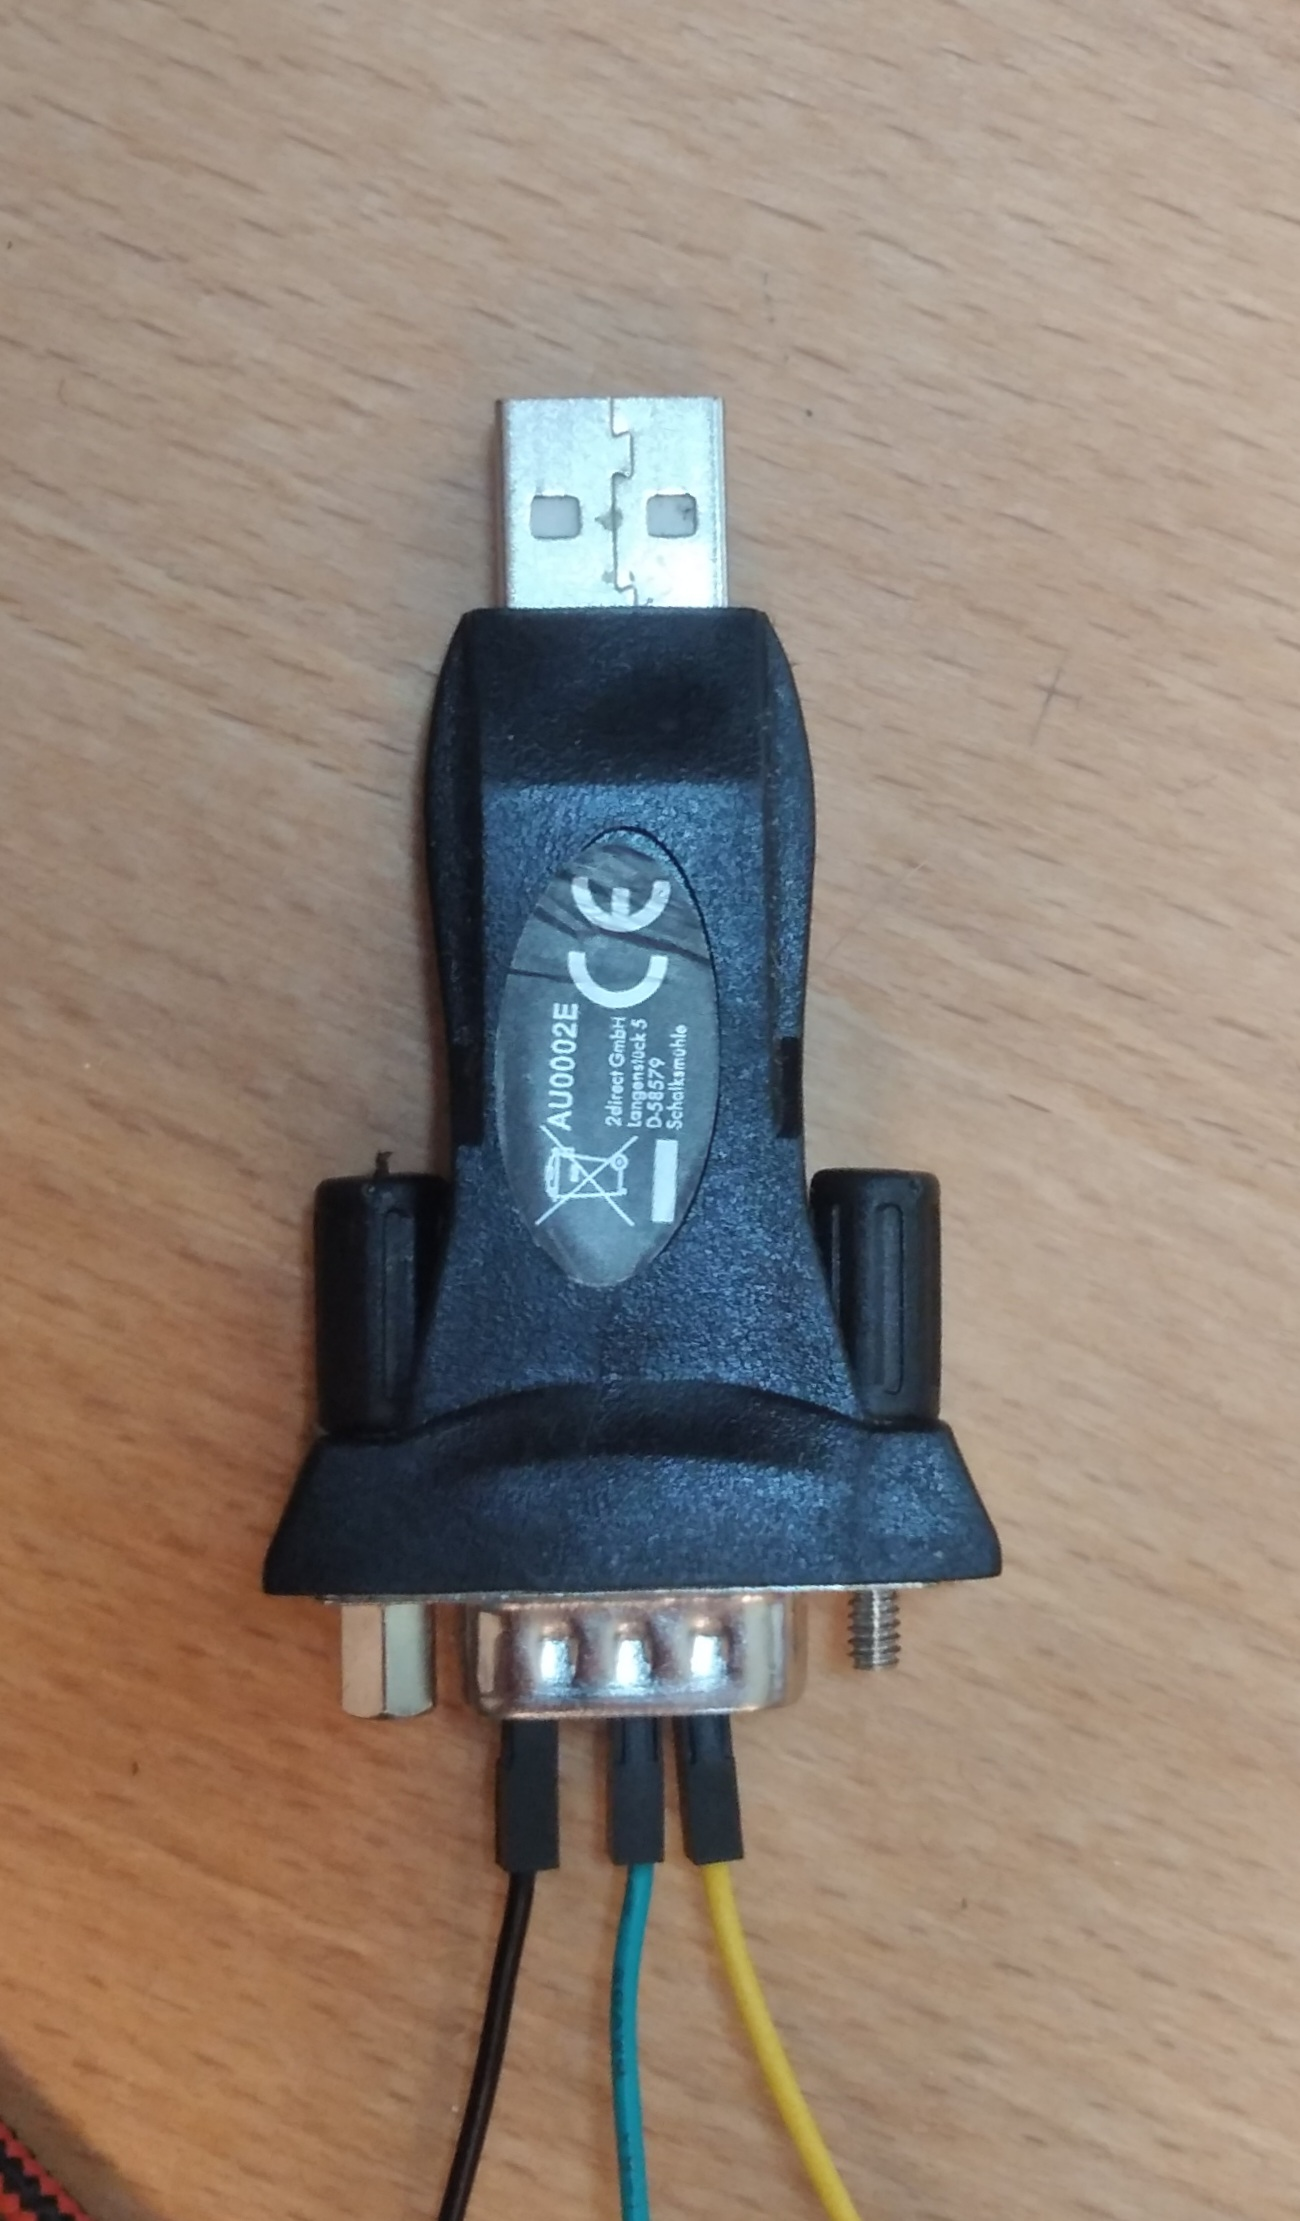
\includegraphics[width=5cm,angle=90]{Geraete/RS232.jpg}}\\
\end{tabular}